\chapter{Results}

All models and the following analyses are provided as .xml files and Jupyter notebooks respectively in the supplementary folder.
\section{Reconstruction of metabolic models and community model creation}
The basis for all my analysis form the reconstructed metabolic models of the two SynComs. Therefore, my first research question that investigates the models in terms of their compliance to community standards is essential. 

Of the total 52 individual strains cultured in vitro, only 50 assembled genomes were available. The reconstruction process yielded 50 models containing 2,559 reactions and 1,676 metabolites on average, distributed across three compartments (cytosol, periplasm and extracellular space).
Evaluation of the MEMOTE reports revealed 8 mass and 961 charge imbalanced reactions (see Table~\ref{tab:curation_imbalances}). MEMOTE differentiates between these imbalances, however a reaction can be flagged as both mass- and charge imbalanced at the same time and will therefore be reported twice. Mass imbalances occur due to different protonation states of metabolites, causing an uneven number of protons on the reactant and product side or are a result of the incomplete resolution of placeholders in compound formulas ($X$ and $R$). The latter explains also why there are more mass imbalances after the automated curation step, which nevertheless decreased the number of charge imbalanced reactions by more than half. Charge imbalances are mainly caused by differing amounts of protons in the chemical formula and the charge state of a metabolite. All in all, through manual curation I achieved stoichiometric consistent models with no mass imbalances and only 82 charge imbalanced reactions (see Table~\ref{tab:curation_imbalances}).

\begin{table}[H]
  \centering
  \caption{Mass and charge imbalances across draft, automated BiGG overwrite, and curated models.}
  \label{tab:curation_imbalances}
  \begin{tabularx}{\linewidth}{Xccc}
    \hline
    \textbf{Metric} & \textbf{Draft models} & \textbf{Post automated BiGG overwrite} & \textbf{Curated models} \\ \hline
    Sum of all mass imbalances across all models & 190 & 2105 & 0 \\
    Total distinct mass imbalances across all models & 8 & 124 & 0 \\
    Sum of all charge imbalances across all models & 22512 & 9622 & 807 \\
    Total distinct charge imbalances across all models & 961 & 453 & 82 \\ \hline
  \end{tabularx}
\end{table}

Further curation steps focused on dead-ends, blocked reactions and removing the duplicates detected by MEMOTE and MACAW. MEMOTE flagged 45 average blocked reactions per model, which are defined as reactions that are not able to carry flux, indicating network gaps. MACAW highlighted further duplicates, which were resolved. Due to the substantial number of blocked reactions and energy-generating cycles and the considerable amount of time required to resolve them, their investigation was beyond the scope of this thesis.

\begin{table}[H]
  \centering
  \caption{Comparison of average model metrics before and after curation}
  \label{tab:average_model_metrics}
  \begin{tabularx}{\linewidth}{Xccc}
    \hline
    \textbf{Metric} & \textbf{Draft models} & \textbf{Curated models} \\ \hline
    Number of reactions per model & 2558.64 & 2536.12 \\
    Number of metabolites per model & 1675.50 & 1671.24 \\
    MEMOTE consistency score all models & 0.58 & 0.93 \\
    MEMOTE final score all models & 0.73 & 0.86 \\ \hline
  \end{tabularx}
\end{table}

Compared to the draft models, the average final MEMOTE score increased by 13\%, and the consistency score improved 35\% (see Table \ref{tab:average_model_metrics}). Unbounded fluxes in the medium and annotation gaps caused the remaining inconsistencies and imperfect scores. Overall the curation efforts clearly improved the structural and metabolic consistency of the models, establishing a robust, standardised foundation for subsequent analyses.
\\


Upon finishing the curation process, the SynComs were assembled using the tool MICOM \cite{diener_micom_2020}. The resulting core community contains $27$ members which accumulate $46{,}468$ metabolites and $70{,}762$ reactions. The resulting trait-optimised community is composed of $26$ members, totaling to $43{,}490$ metabolites and $65{,}177$ reactions. This large number of objects is due to MICOM's compartmentalisation strategy, where each metabolite and reaction is specific to the compartment and strain it is built in. For example, intracellular glucose is formatted as \texttt{glc\_\_D\_c\_\_\{strain\_id\}} instead of \texttt{glc\_\_D\_c}. Condensing the reactions and metabolites by compartment and strain, HvSC1 contains $5{,}293$ unique reactions and $1{,}622$ unique metabolites, whereas HvSC2 contains $5{,}455$ reactions and $1{,}667$ metabolites.


\section{Choice of the optimisation method}
To obtain the communities’ metabolic fluxes, which are the basis for all subsequent analysis steps, I optimised the models for community growth. Furthermore, testing growth is one way to evaluate model quality, directly addressing my first research question. During my simulations, I tested different optimisation methods that are included within the MICOM package (Section \ref{sec:MICOM}). This investigation was primarily motivated by improbable results observed in one experiment: when applying \texttt{cooperative\_tradeoff()}, across all trade-off values $\alpha$, artificially blocking sugar exchanges within the community resulted in higher overall community growth rates compared to scenarios where sugar secretion was allowed. This outcome does not align with the basic assumptions of constraint-based modelling, as removal of a constraint (block of the secretion) expands the feasible flux space, which can not have a lower global optimum than a constrained subset. Therefore, the community growth rate should be equal or lower for additional constraints, never higher. This error did not occur when using the standard \texttt{optimise()} objective function. 
\\


The discrepancy led to a more detailed systematic evaluation and comparison of MICOM's underlying optimisation strategies. The \texttt{optimise()} method consistently yields the highest total community growth rate across all tested methods. However, it also results in the highest number of non-growing strains within the community. Furthermore, under this strategy I observed non-growing strains which still carried active metabolic fluxes. Biologically this result is unrealistic as these strains are used as passive, extracellular extensions of active strains rather than distinct living organisms. This underlines the need for further regularisation of growth rates, as done with the trade-off strategy. 
To mitigate these problems caused by MICOM’s optimisation function, I introduced a custom trade-off function, which is based on MICOM's \texttt{cooperative\_tradeoff()}, see Section \ref{sec:MICOM}, but bypasses the crossover strategy and accepts non-optimal, yet numeric results (see Table \ref{tab:solution_statuses}). 


\section{Comparison of community and individual growth rates}
The predicted growth of a model is one indicator of its quality. Therefore, to answer the first research question, I assessed the individual strain and the community growth in their native environment: the barley apoplastic fluid. None of the models showed growth in monoculture on the apoplastic medium, highlighting the significance of community interactions in enabling growth. 
\\


In the community context, the core community exhibits higher growth rates ($\mu_{c1} = 7.534 \text{h}^{-1}$ vs. $\mu_{c2} = 5.945 \text{h}^{-1}$), as well as higher growth rates among its members. Median individual growth rates are higher in HvSC1 ($\mu_{i,\text{median}} = 0.236\,\text{h}^{-1}$) than in HvSC2 ($\mu_{i,\text{median}} = 0.212\,\text{h}^{-1}$). While this difference may seem minor, the clustering of the individual values around this median differs noticeably: HvSC1 growth rates are far more tightly clustered around the median (IQR: 0.04), whereas HvSC2 spanned a much wider range (IQR 0.09) (Fig.~\ref{fig:growth_comparison}). 
The three taxa present in both communities consistently grow stronger in the core community (see green coloured strains in Fig.~\ref{fig:growth_comparison}), which shows that the difference in community growth rate can not only be attributed to differences in taxa composition but also community interactions. This pattern is underlined by taxa with small growth rates. Only one strain in HvSC1, namely 1124, grows less than $0.1\,\text{h}^{-1}$, compared to four taxa in HvSC2. Growth in the core community is both higher on average and generally more evenly distributed, with smaller differences in individual growth rates compared to the trait-optimised community.

\begin{figure}[H]
  \centering
  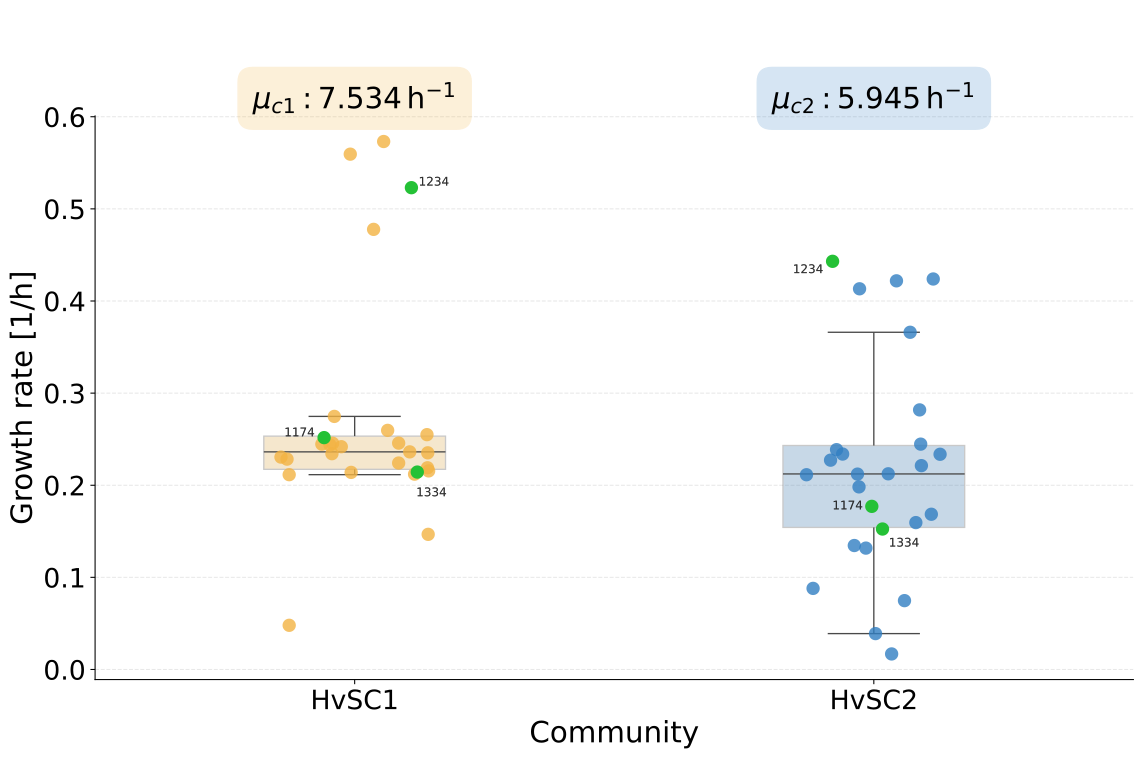
\includegraphics[width=1\textwidth]{fig/Individual_growthrates_boxplot_l2pfba_labels.png}
  \caption[Comparison of individual taxon growth rates by community on completed apoplastic fluid medium]{Comparison of individual taxon growth rates by community on completed apoplastic fluid medium. Community is indicated by colour: HvSC1 (yellow) and HvSC2 (blue). Green strains occur in both communities. HvSC1 shows higher community growth $\mu_c$ as well as higher average individual growth rates $\mu_i$, which are also more centered around the median, compared to HvSC2.}
  \label{fig:growth_comparison}
\end{figure}

\section{Metabolic profiles of each community}
To understand the metabolic requirements of each community, their internal niche overlap as well as the cross-feeding within a community, and thus answer the second research question, I analysed the uptake and secretion profiles of each community. These I obtained from growth simulations on the completed apoplastic fluid medium. Both communities take up 42 metabolites from the apoplastic medium, of which 40 are shared between the communities. These include amino acids, sugars as well as inorganic ions and provide the basis for growth. HvSC1 exclusively takes up UDP-N-acetyl-D-glucosamine, and HvSC2 exclusively utilises succinate. Beyond these medium-derived uptakes, the majority of uptake reactions (488 in HvSC1 and 504 in HvSC2) correspond to metabolites not present in the medium and thus are cross-fed metabolites between community members.
\subsection{Niche overlap}
Based on the collective uptakes of each community, I assessed their metabolic niche. The core community exhibits a larger niche overlap compared to the trait-optimised community, as shown by the higher MRO score, increased co-consumption (Fig. \ref{fig:combinednumbercoconsumptionsheatmap}) and smaller number of metabolites taken up only by a small fraction of the community (Table \ref{tab:metabolic_profiles}). This is in line with the larger number of metabolites exchanged in the native community, showing that the nutritional requirements within the community overlap more, reflecting their common co-occurrence, while the other community's nutritional requirements are more diverse.
As the range of possible uptakes from the medium was already limited due to the medium composition, no other clear metabolic niches became apparent. Other differences in metabolic profiles are therefore primarily caused by differences in cross-feeding behaviour.

\begin{table}[H]
  \centering
  \caption{Comparison of community interaction metrics for HvSC1 and HvSC2.}
  \label{tab:metabolic_profiles}
  \begin{tabularx}{\linewidth}{Xccc}
    \hline
    \textbf{Metric} & \textbf{HvSC1} & \textbf{HvSC2} \\ \hline
    Average number of co-consumed metabolites for each taxon pair & 43 & 39 \\
    MRO score & 0.512 & 0.501 \\
    MIP & 0.911 & 0.914 \\
    fMIP & 0.376 & 0.469 \\
    Average number of exchanged metabolites for each taxon pair & 15.060 (SD 11.003) & 12.378 (SD 8.414) \\
    Average sum of fluxes per pair & 1.974 (SD 2.186) & 3.846 (SD 3.561) \\
    Number of metabolites taken up by five members or less & 224 & 275 \\ \hline
  \end{tabularx}
\end{table}

\subsection{Metabolic interactions within the communities}
\subsubsection{Metrics in pairwise interactions}
Both communities show extensive amounts of cross-feeding, covering more than 90\% of their required metabolite range through community interactions (MIP score). However, while the potential range of shared metabolites (MIP) is nearly identical between the two communities, the flux volume through these pathways (fMIP) differs. Community interactions account for almost half of the total uptake fluxes in the trait-optimised community, whereas the more than 60\% of the core communities' uptakes stem from medium uptakes. Thus, while both communities share a similar diversity of cross-fed compounds, HvSC2 routes a larger magnitude of its overall metabolic flux through these community exchanges (Table \ref{tab:metabolic_profiles}).

An evaluation of pair-wise interactions within the communities underlines this result: The total sum of exchanged fluxes is higher in HvSC2 than in HvSC1 (Fig. \ref{fig:absolut_metaboliteinteractions}A, B). Strain 709 stands out, as it shares relatively high exchange fluxes with almost all members of HvSC2. This is not mirrored in the diversity of its exchanges: the total number of distinct exchanges is generally lower across HvSC2. Conversely, HvSC1 relies on a broader range of smaller exchanges, with Strains 892 and 1334 exchanging numerous different metabolites with fellow community members (Fig. \ref{fig:absolut_metaboliteinteractions}C).
\\


Importantly, interaction frequency does not directly scale with flux volume. High cumulative flux in the communities stems either from many minor exchanges or a few high-magnitude interactions. Overall, HvSC1 exchanges more metabolites distributed across smaller fluxes and wider spanned across the community. HvSC2 features less exchanged metabolites but a substantially higher flux volumes per interaction.
\begin{figure}[H]
	\centering
	
\includegraphics[width=1\linewidth]{fig/Combined_nex_sumflux_heatmap}
	\caption[Pairwise metabolic interaction in absolute numbers]{Pairwise metabolic interaction in absolute numbers. The heatmaps show pairwise cross-feeding interactions in scope of  magnitude (A, B) and number of exchanged metabolites (C, D). While HvSC1 is generally exchanges more metabolites, HvSC2 exhibits higher fluxes in its exchanges.}
	\label{fig:absolut_metaboliteinteractions}
\end{figure}


\subsubsection{Symmetry in metabolic interactions}
HvSC1 exhibits greater network connectedness, averaging more exchanged metabolites per strain pair, but with lower and more symmetric exchange fluxes. Symmetric exchange fluxes mean, that in a pairwise interaction assessment partner X provides the same flux amount as partner Y.  Based on flux magnitudes, no clear donor-only or recipient-only strains can be identified in HvSC1 (Fig. \ref{fig:balance_metabolicexchanges}A). In contrast, exchange fluxes in HvSC2 are heavily asymmetric: Strain 709 dominates flux magnitude as a major provider of amino acids and ethanol, while strains 1101 and 939 stand out as key providers of nucleotides, thiamine, and ammonium (Fig. \ref{fig:balance_metabolicexchanges}B). The symmetry in the number of exchanged metabolites follows the opposite pattern between the communities. In HvSC1 the group of strains 100, 1167, 1391, 163, 230, and 2774 stands out as wide-range providers. Notably, strains 1334 and 892 cross-feed with all community members in highly diverse metabolite exchanges (Fig. \ref{fig:balance_metabolicexchanges}D). HvSC2 is overall more symmetric, and therefore more balanced in the diversity of its exchanges, even though its flux magnitudes are heavily donor-driven.
This contrast highlights that the core community is more metabolically interdependent and reciprocal in flux exchange, relying on a distributed network of strains rather than a single donor strain.

\begin{figure}[H]
	\centering
	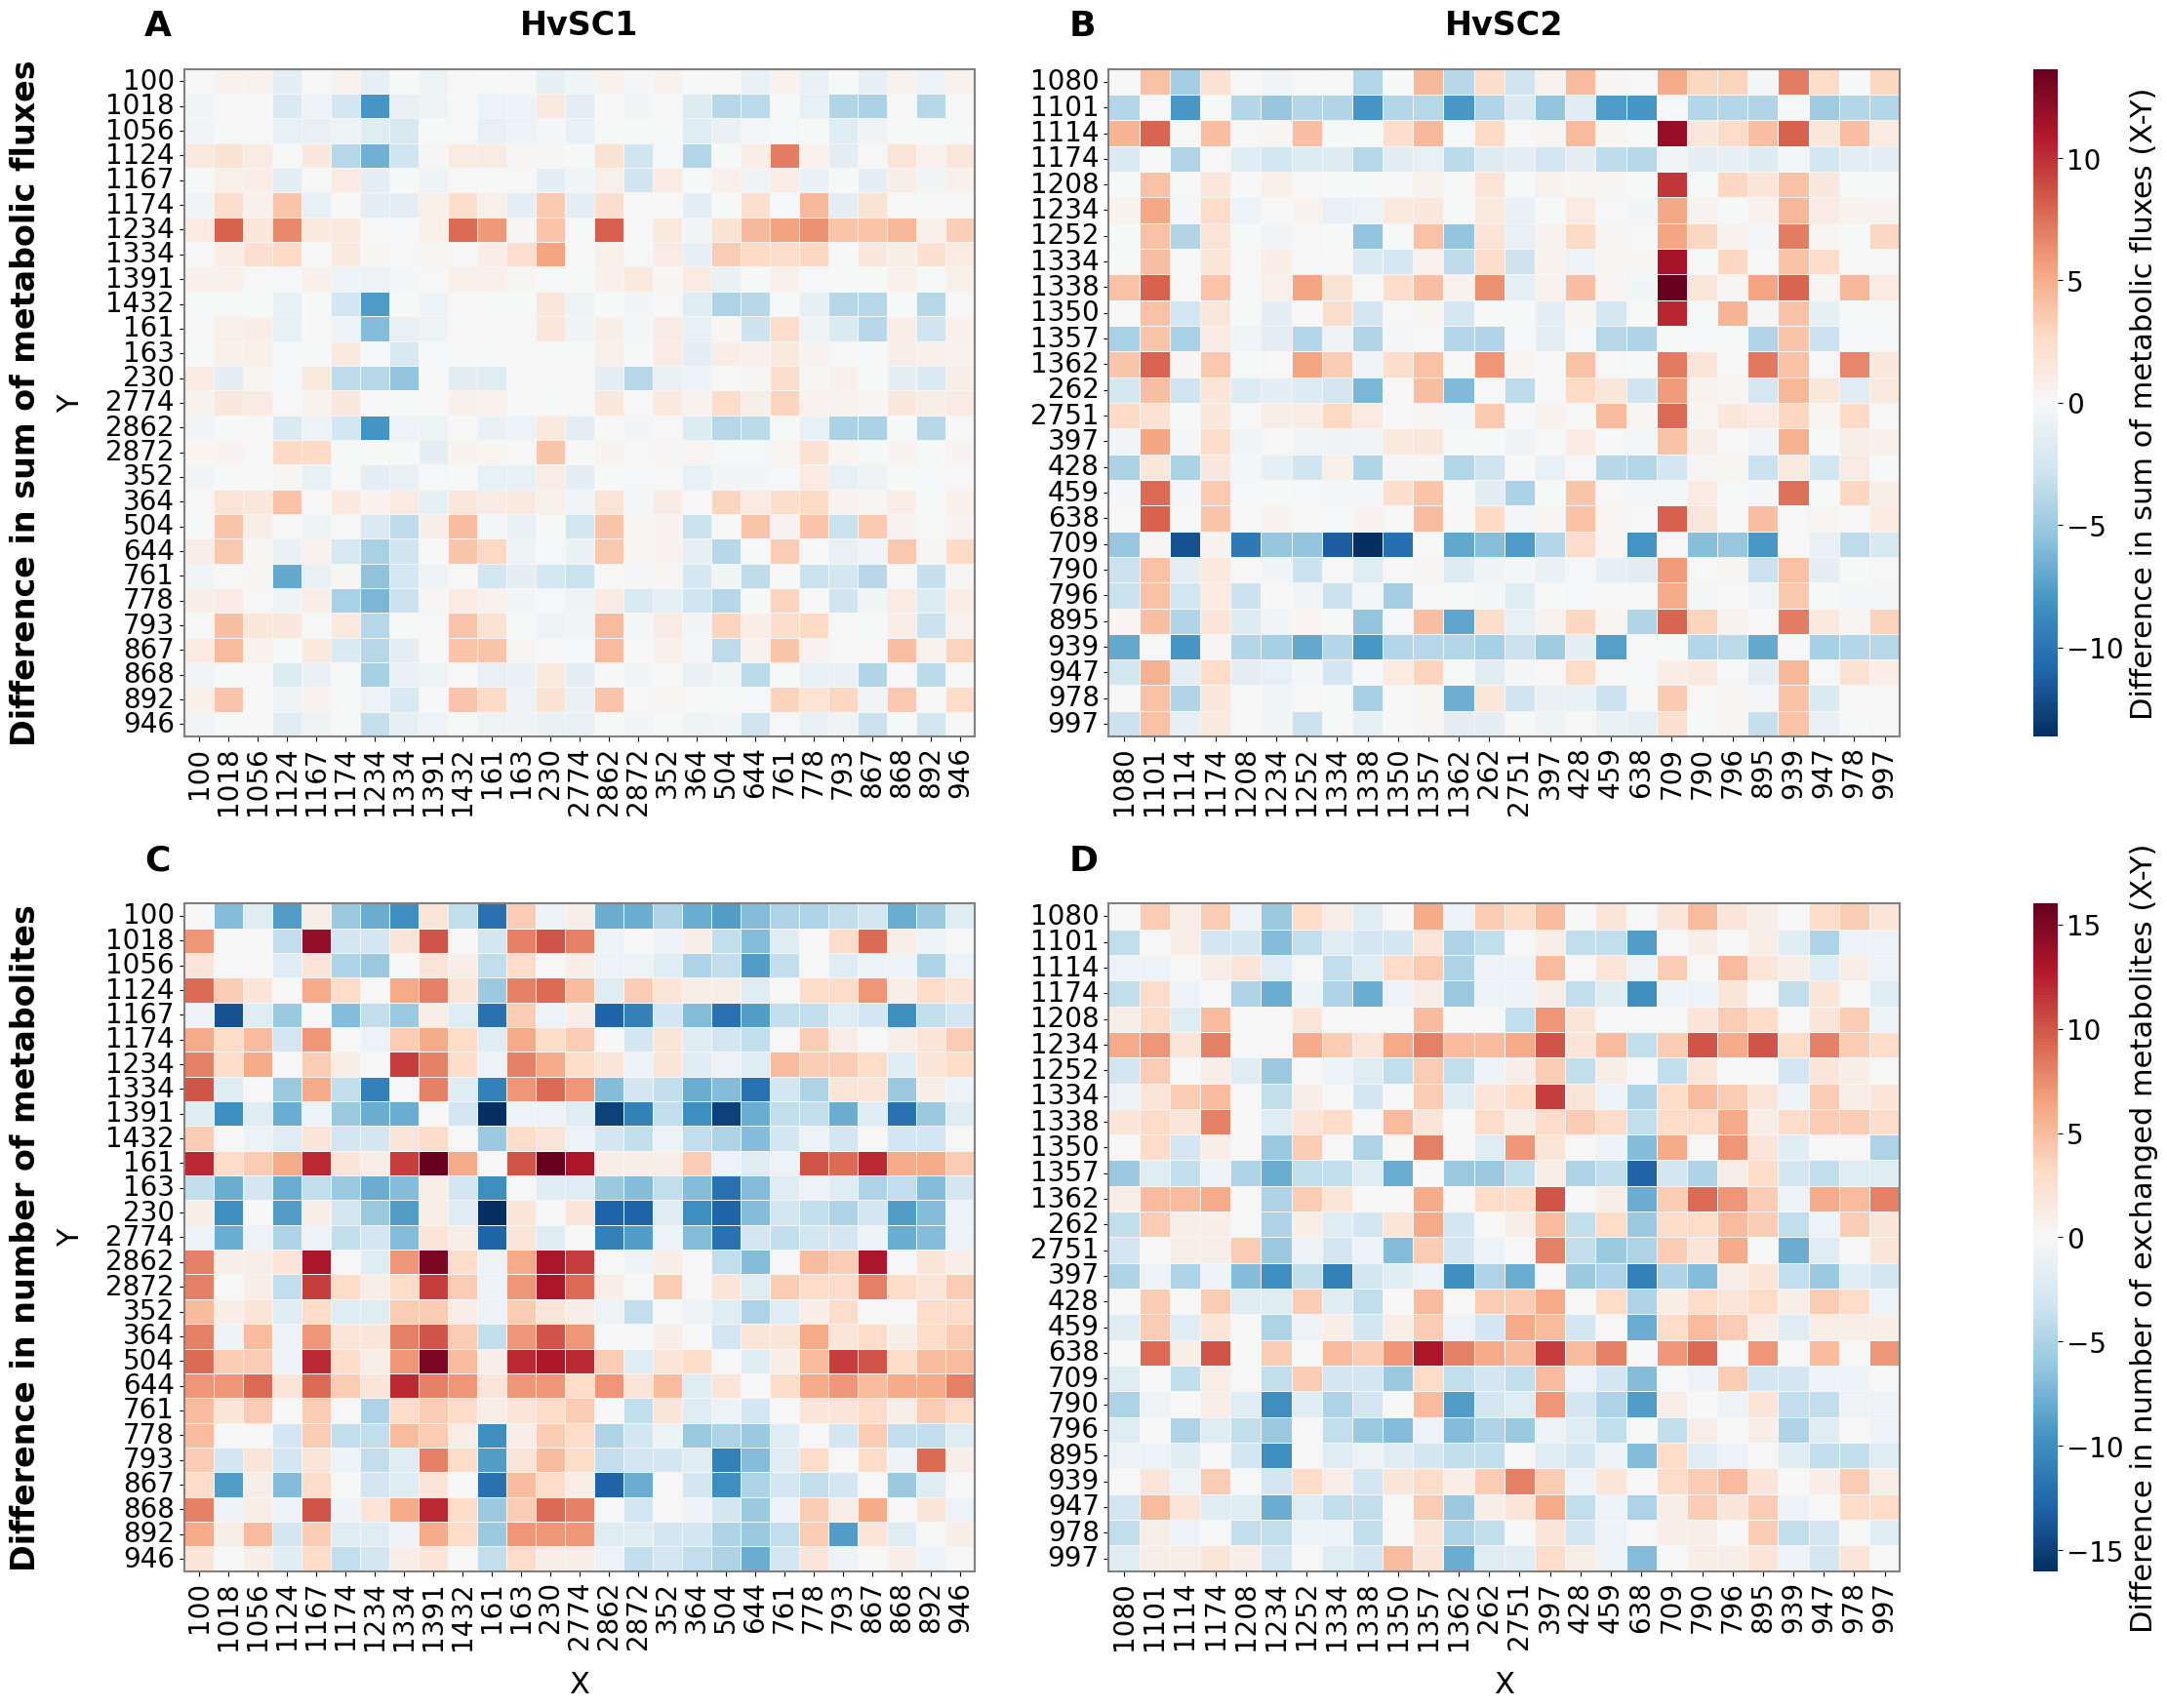
\includegraphics[width=1\linewidth]{fig/Combined_balance_nmets_flux_heatmap}
	\caption[Symmetry of pairwise metabolic interactions]{Symmetry of pairwise metabolic interactions. The heatmaps show pairwise cross-feeding interactions in scope of magnitude (A, B) and number of exchanged metabolites (C, D). HvSC1 is more asymmetric in the number of exchanged metabolites but exhibits higher symmetry in the exchanged metabolic fluxes compared to HvSC2.}
	\label{fig:balance_metabolicexchanges}
\end{figure}

\section{Drop-out experiments}
Previous analyses showed that both communities rely heavily on metabolic exchanges and indicate certain strains that might hold special importance in community structure. This raises the question how the removal of individual strains affects community behaviour. Therefore, to address my third research question, I generated drop-out communities by removing one member at a time and examined resulting changes in community and individual growth rates. 
\\


\begin{figure}[H]
  \centering
  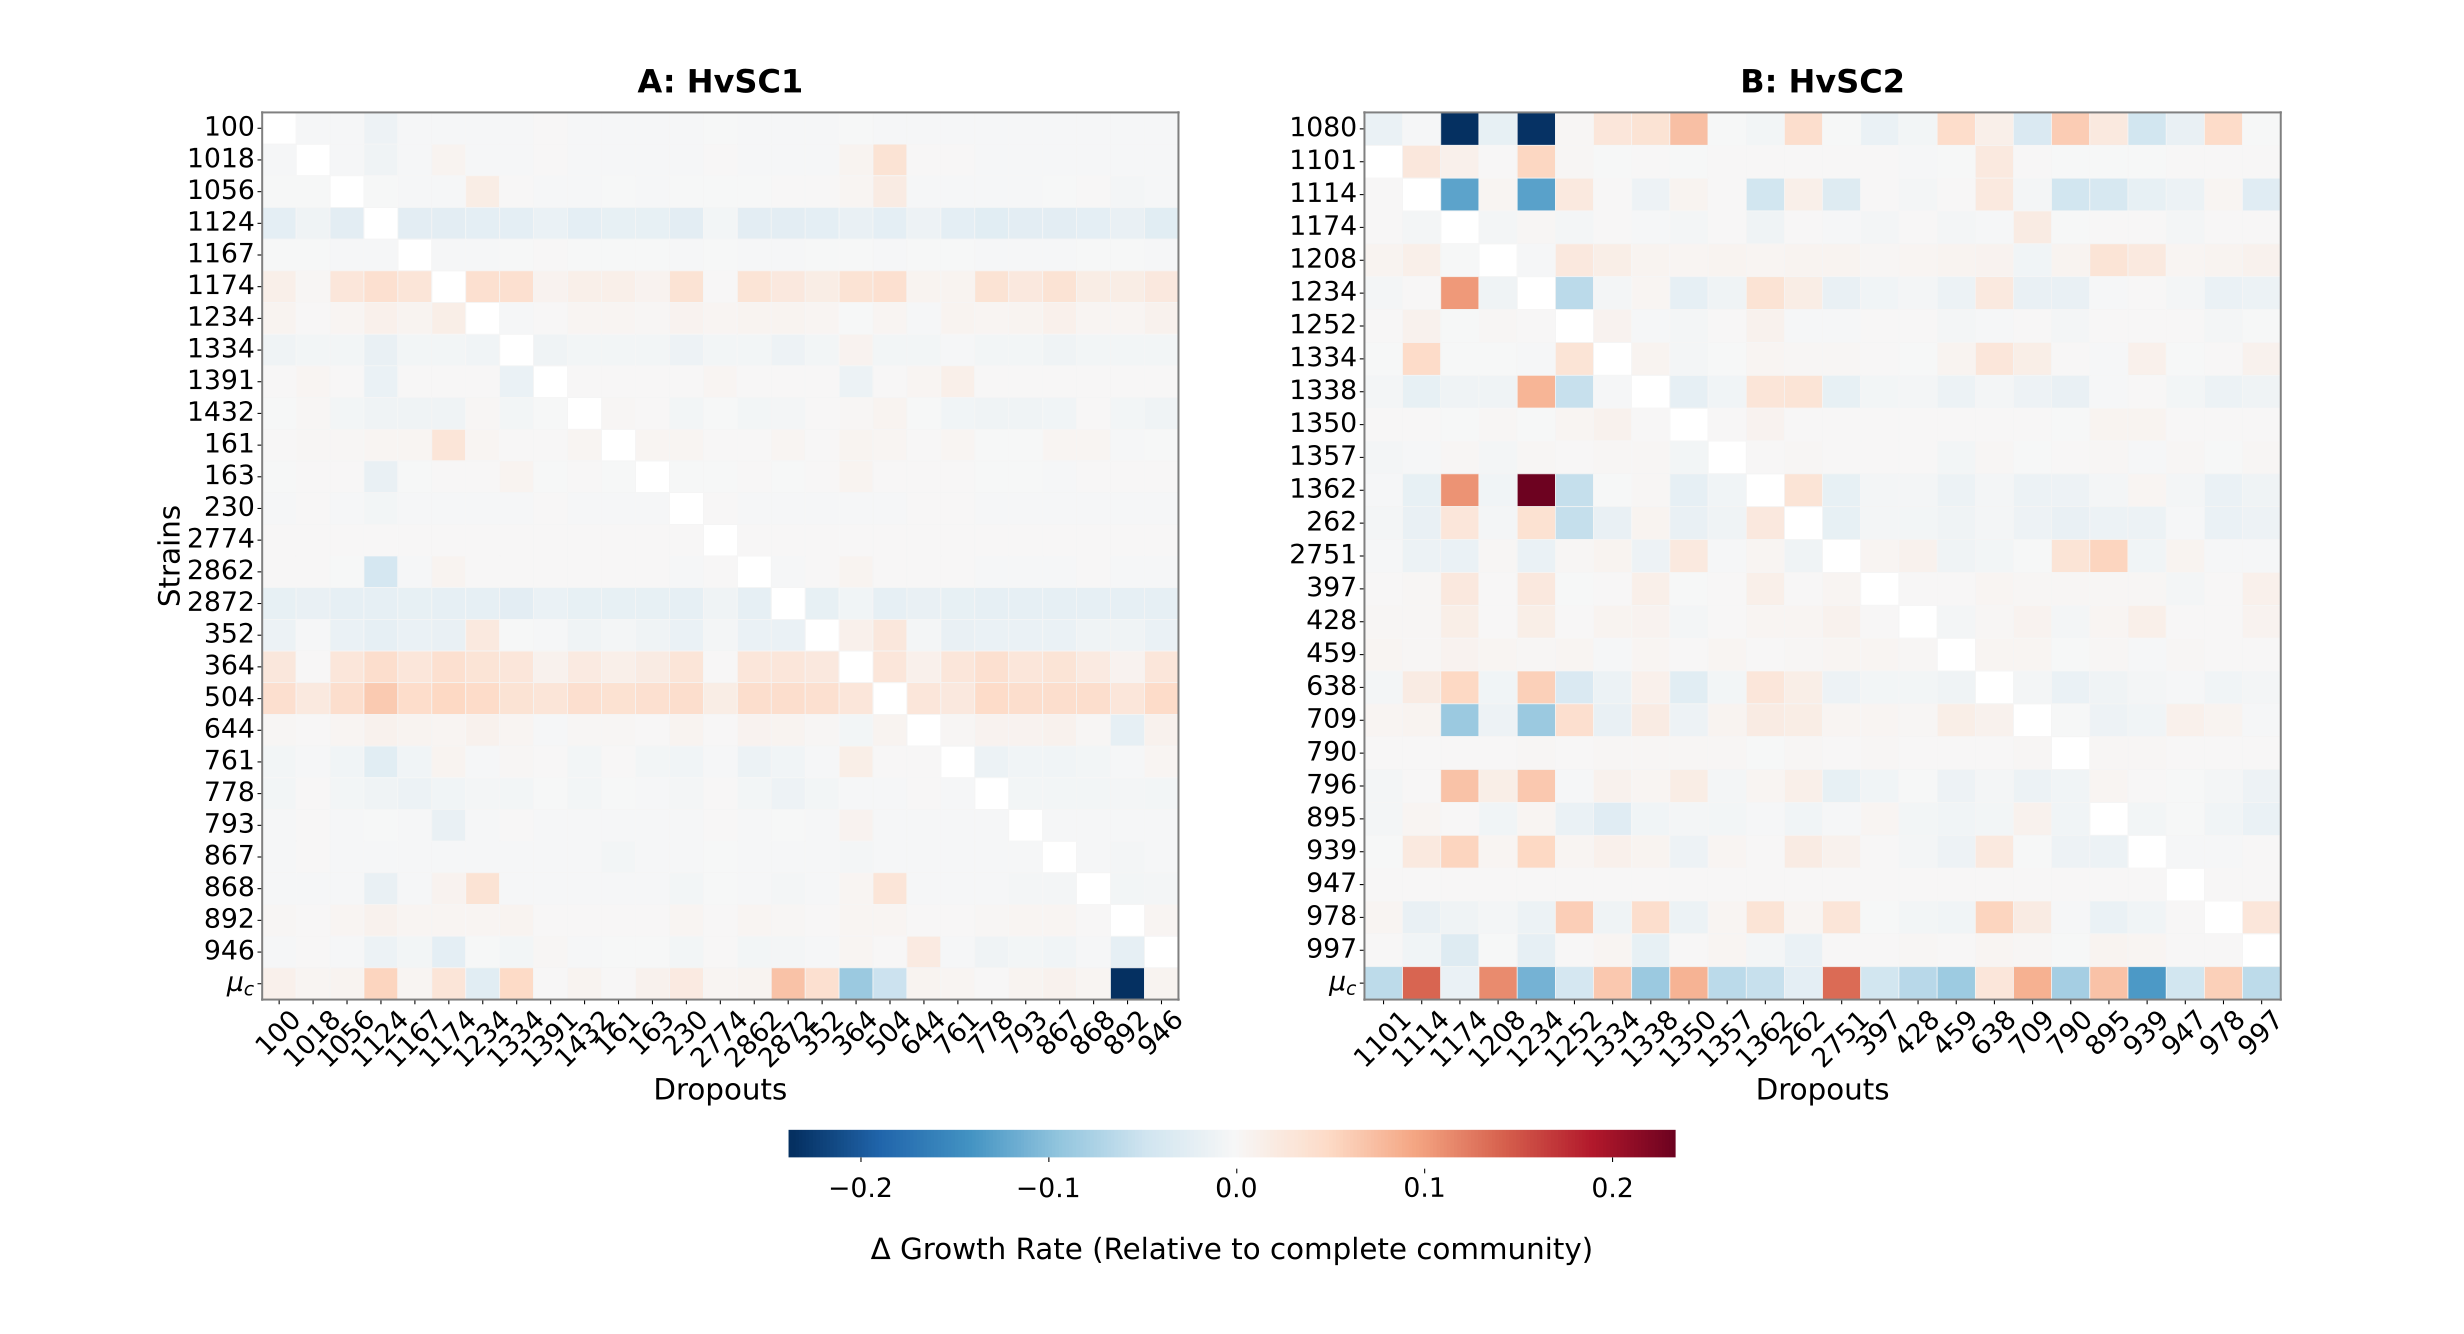
\includegraphics[width=1\textwidth]{fig/Dropout_growthrates.png}
  \caption[Impact of single-strain drop-outs on strain-level and community growth rates]{Impact of single-strain drop-outs on strain-level and community growth rates. Heatmaps for (A) HvSC1 and (B) HvSC2 display the change in growth rate ($\Delta$ Growth Rate) relative to the complete community baseline. Individually removed strains are listed on the x-axis, while remaining strains are shown on the y-axis. The bottom row ($\mu_c$) displays the net effect of each drop-out on overall community growth. Red hues indicate increased growth rates relative to the complete community, blue hues indicate reduced growth rates.}
  \label{fig:dropout_growth}
\end{figure}
The core community’s growth decreases by 5\% upon the removal of strain 892. Aside from strain 892, individual drop-outs had minimal impact on HvSC1's community growth. In contrast, the growth rate of the trait-optimised community (HvSC2) fluctuated largely depending on which species was removed (Fig. \ref{fig:dropout_growth}B, bottom row). In HvSC1, a subset of strains stands out by consistently responding to any member's removal compared to the complete community: strains 1174, 364 and 504 always grew more, whereas 1124 and 2872 grew less. No such generalised strains are detected in HvSC2 and its individual strain growth is very little affected by single-strain drop-outs. HvSC2 exhibits wider spread pairwise dependencies. In particular strains 1174 and 1234 displayed strong antagonism toward strains 1362 and 796, and cooperative interactions with strains 1080 and 1114. 
Overall, the drop-out experiments show that the core community is, under the exclusion of its keystone 892, less reliant on the presence of a single strain than the trait-optimised community, which’s growth rate fluctuates notably upon single-strain removal.

\subsection{Potential keystone strain 892}
Since I identified strain 892 as a potential keystone species in the drop-out experiments, I further analysed its metabolic interactions within HvSC1. Strain 892 engages in a total of 563 metabolic interactions within the community, which make up 5.32\% of all community interactions. It exclusively secretes two siderophores (Ferroxamine and Mycobactin T), among aromatic ring derivatives and pH regulating compounds (3-Oxoadipate and 2-Dehydro-D-gluconate). To the 26 fellow members of its community 892 provides a total of 47 metabolites, from which nitrate, aromatic nitro compounds, arginine, protoheme, and acetaldehyde are most frequently exchanged. In return, it accepts CO2 from all other community members as well as glycine betaine, cysteine, nitrite and ammonium. 
To test if 892 could stabilise the growth of the trait-optimised community, I performed a drop-in experiment, introducing 892 into HvSC2. The drop-in increased community growth rate by 8\%, to 6.437$\text{h}^{-1}$. Median individual growth rate did not change, rather the values spread more widely across the whole range, clustering less around the median and more toward the extremes ($IQR_{HvSC2} = 0.089$, $IQR_{Drop-In} = 0.172$) (Fig. \ref{fig:dropin_growth}). This indicates that the addition of 892 benefits only a subset of the community while limiting others.
\\



\begin{figure}[H]
  \centering
  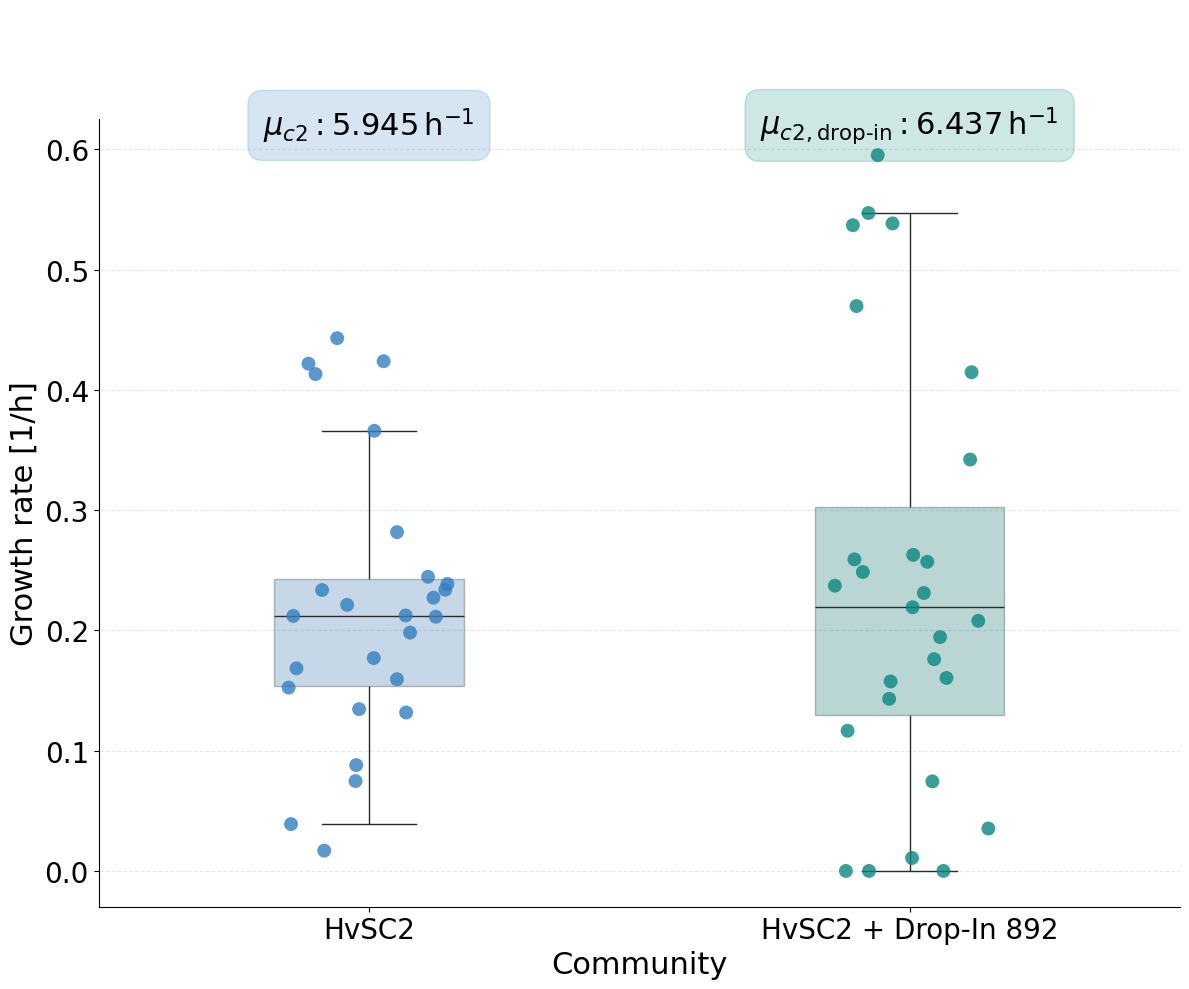
\includegraphics[width=1\textwidth]{fig/DROPIN892_Individual_growthrates_boxplot_l2pfba.png}
  \caption[Impact of drop-in strain 892 on HvSC2's growth]{Impact of drop-in strain 892 on HvSC2's growth. Comparison of individual taxon growth rates HvSC2 and HvSC2 + 892 (Drop-In 892) on completed apoplastic fluid medium. Community is indicated by colour: HvSC2 (blue) and Drop-In (dark green). HvSC2+ Drop-In 892 shows higher community growth rate $\mu_{c2, \text{drop-in}}$ compared to $\mu_2$, but growth rates are more spread, showing that the drop-in only benefits a subset of HvSC2's members.}
  \label{fig:dropin_growth}
\end{figure}

I analysed the metabolic interactions of 892 within the drop-in community, to find potential key metabolite exchanges underlying this altered growth behaviour. The metrics quantifying metabolic interactions changed only slightly (MRO: -0.003, MIP: +0.002, fMIP: +0.005).  Within the drop-in community, 892 engages in a total of 122 interactions and provides 11 metabolites, of which acetaldehyde, L-glutamate, ammonium, and nitrate are most frequently received. However, the strains receiving the highest number of metabolites or the largest total flux are not necessarily those that grow best, indicating that the observed improvement in growth cannot be attributed to metabolic exchange alone.
All in all, introducing strain 892 to the trait-optimised community increased overall community growth but made growth more imbalanced across members, an effect which can not be fully explained by 892's metabolic exchange patterns. 